This thesis investigates stellar streams originating from globular clusters in the Milky Way. Stellar streams are long, thin structures composed of stars that have escaped a host stellar system, forming coherent tails that can span large regions of the sky. Globular clusters are dense gravitationally bound systems containing hundreds of thousands to millions of stars. They are one source of stellar streams. In Chapter 4, I present our study in which we simulated the expected distribution of stellar streams originating from the entire Milky Way globular cluster system. This study was the first of its kind. Stellar streams have high hopes for being inferential tools for inferreing the presence of dark matter sub halos within the Galaxy. These halos may perturb the stellar streams leaving ``gaps'' in their wake. In Chapter~5, we explored how the collective gravitational influence of all globular clusters can also perturb produce such gaps.

The structure of the thesis is as follows. The remainder of the introduction provides background on stellar streams, globular clusters, and their astrophysical context, as well as an overview of the current state of the field. Chapter~2 outlines the physical framework used to model stream formation and interpret their morphology. Chapter~3 describes the numerical methods employed in the simulations, including convergence tests and estimates of computational cost. Chapters~4 and~5 present two published studies, with the final chapter discussing these results in the broader context of the literature and highlighting future directions.

\section{General context}
    Before explaining why Milky Way globular clusters and stellar streams are scientifically interesting, it is important to first set the scene. This thesis fits neatly within the field of galactic astronomy, which, at its core, studies the current state of our galaxy and the processes that shaped its formation within the broader context of the universe.

    If we start this narrative from the beginning and place stellar streams and globular clusters in the timeline of cosmic history, their importance becomes clearer. The story begins best at the very start. The Lambda Cold Dark Matter ($\Lambda$CDM) cosmological model is currently the leading theory of the universe, successfully unifying a variety of observational evidence—from the Cosmic Microwave Background Radiation and the large-scale distribution of galaxies to the accelerating expansion of the universe \citep{2001LRR.....4....1C,2022NewAR..9501659P}.

    Shortly after the Big Bang, conditions allowed protons, neutrons, and electrons to form and interact. For a few minutes, these particles collided and fused into heavier elements in a process known as Big Bang Nucleosynthesis \citep{2007ARNPS..57..463S}. When this phase ended, the universe's composition was mostly hydrogen, deuterium ($^2$H), helium-4 ($^4$He), and trace amounts of helium-3 ($^3$He) and lithium-7 ($^7$Li). By mass, hydrogen made up roughly 75\%, and helium about 25\% of the primordial universe \citep{1966ApJ...146..542P,2016RvMP...88a5004C}.

    Dark matter, which accounts for about five times more mass than ordinary matter, played a critical role in structure formation \citep{2020A&A...641A...6P}. In the early universe, dark matter was distributed nearly uniformly but developed gravitational instabilities that caused it to collapse into a cosmic web of filaments and nodes. These massive nodes created deep gravitational wells that attracted ordinary matter \citep{1974ApJ...187..425P}. The infalling gas subsequently cooled and formed stars. The resulting complex of stars, gas, and dark matter constitutes a galaxy \citep{2008LNP...740.....P,2010gfe..book.....M}.

    Galaxies contain stars that are born, fuse hydrogen and helium into heavier elements, and eventually die—often as supernovae—enriching the interstellar medium with these heavier elements \citep{2019A&ARv..27....3M}. This process is a strong function of cosmic time as the chemical evolution of the universe becomes more metal rich. For example the first generation of stars, known as Population III (Pop III) stars\footnote{Stellar populations are named in reverse order of discovery. The first population identified corresponds to stars in the local solar neighborhood, which include third-generation stars or higher. Population II stars are second-generation, while Population III are the very first stars in the universe.}, formed in a very different environment, one devoid of metals \citep{2002Sci...295...93A, 2005SSRv..117..445G, 2013RPPh...76k2901B}. The chemical composition of the gas is crucial since it influences the initial mass function (IMF) of stars. Stars formed from pristine, metal-free gas tend to have a top-heavy IMF, favoring the formation of massive stars \citep{2002ApJ...571...30S,2006MNRAS.369..825S}. In contrast, even small amounts of metals introduced into the gas can dramatically shift the IMF toward the formation of lighter stars \citep{2021MNRAS.508.4175C}.

    \citep{2015ARA&A..53...51S} provides a review discussing galaxy evolution. It has everything from merger trees to chemical enrichment as a function of redshift.  


    -   \citet{2025arXiv250116438K} is laying out a great review for globular cluster formation \dots

    - so efficient that the formation of the N stars must have happened within one dynamical crossing time (what was the paper that said this?)

    - globular clusters are also incredibly interesting becuase of their old ages 

    - in fact it was one of the first ways we were able to date the age of the universe. 

    - Paolo Padoan, Raul Jimenez, Jones proposed a path way to form proto clusters. 

    - Aarseth wrote ``on the collapse and violent relaxation of protoglobular clustres'' 1987

    When stars are made, in many circumstances, they may not just form single stars but clusters of stars. These star clusters come to be when many stars form at once and are also bound to each other gravitationally. One of the most essential objects in this thesis is globular clusters, which are clusters containing hundreds of thousands to millions of stars. 

    \citet{1988ApJ...324..288A} talks about the conditions for globular clusters to form. He states that the fragmentation process must be efficient since the spread in iron abundance is small, therefore all the stars formed within once crossing time. 


    These star clusters, or any extended object that orbits around a larger host, experience tidal forces. There are many examples of this in nature. The most familiar example is how the lunar tides control the water. But for this work, we are interested in more extreme tidal forces, those that are strong enough to disintegrate a body. For example, some hypotheses say that Saturn's rings come from a body that was ripped apart by Saturn's tidal field and then became a collection of rocks and dust \citep{2009Icar..199..413C}. Also, tidal forces played a pivotal role in the Earth-Moon formation scenario; an excellent visualization of the  code SWIFT \url{https://swift.strw.leidenuniv.nl/about.html} \citep{2024MNRAS.530.2378S}, as the proto-moon came to close to the earth, the tidal forces disintegrated it, the earth absorbed a portion and a portion distanced itself from the world to create the moon.

    Those are examples in which the tidal forces rip apart solid bodies. However, star clusters are not solid objects but are instead composed of many stars that are bound together gravitationally. The tidal forces disintegrate star clusters in a much more gentle way. The tidal forces inject enough energy to gently and slowly pull the cluster apart. A result is that the stars that escape from the cluster have more or less the same orbit as the cluster's center of mass \citep{1972ApJ...178..623T,1995AJ....109.2553G}. As the system moves along, the stars coherently spread out along one orbital trajectory and create stellar streams. See Fig.~\ref{fig:S5MilkywayStreams}. 

    \begin{figure}
        \centering
        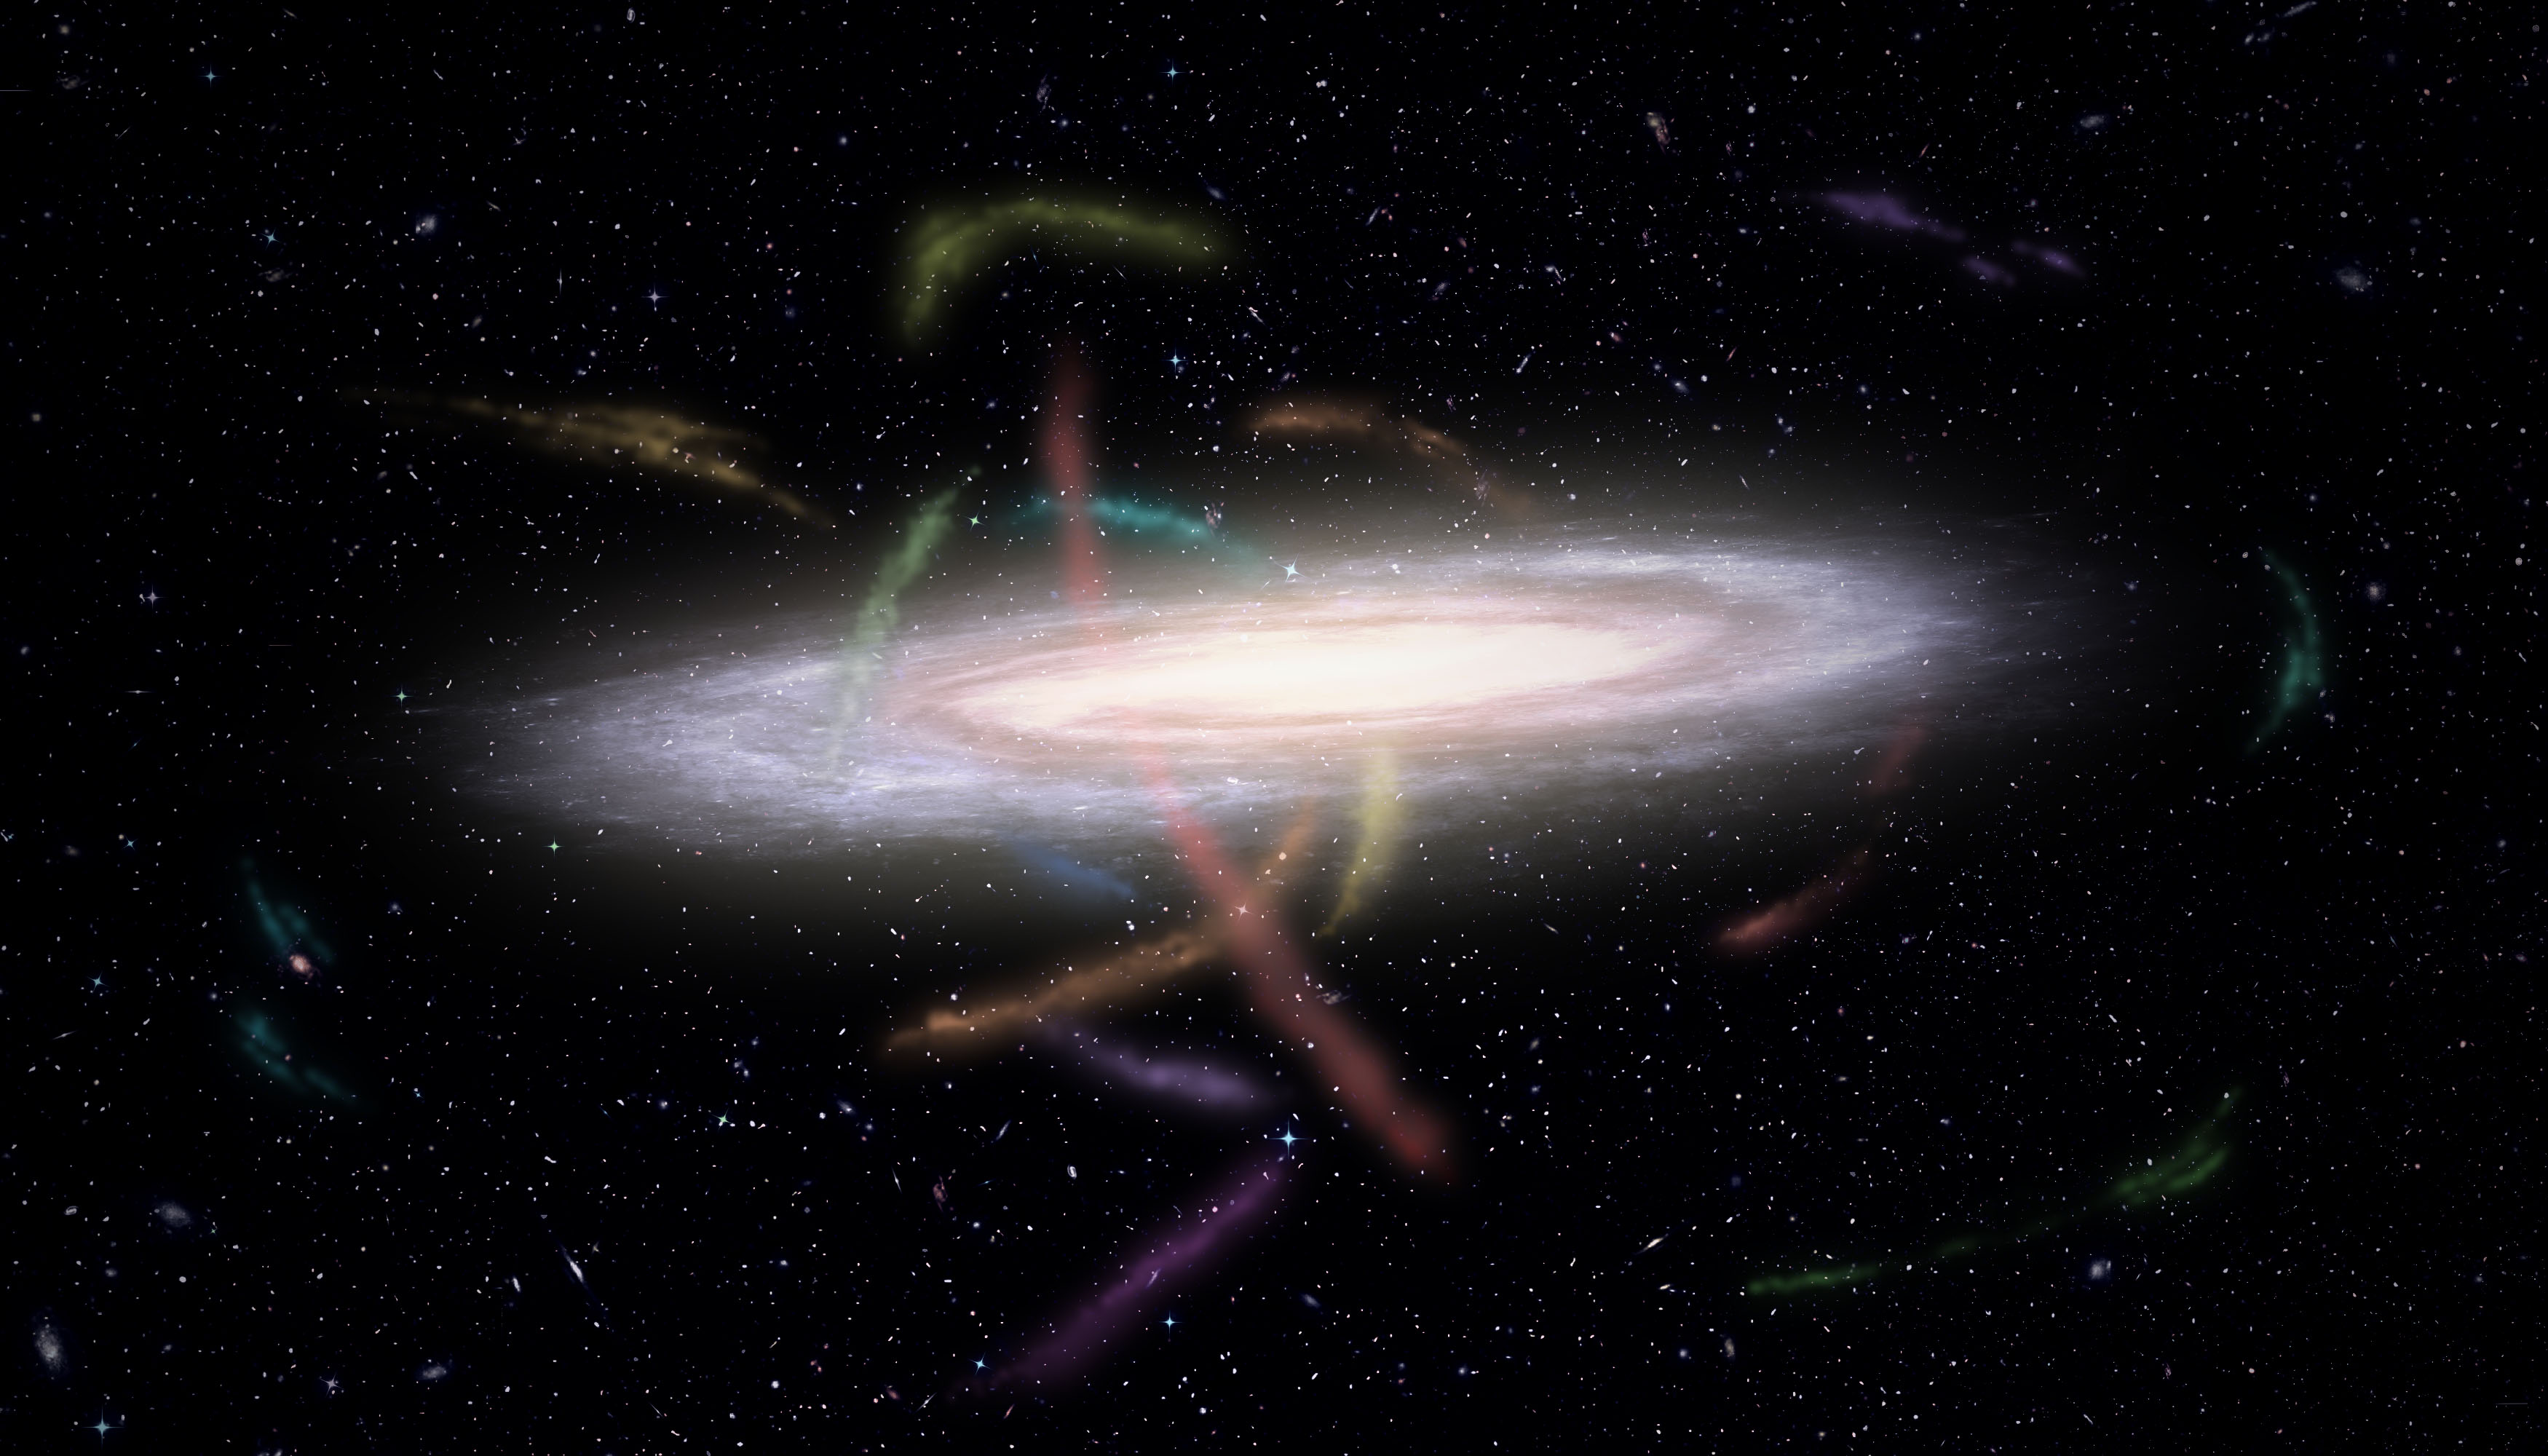
\includegraphics[width=\linewidth]{images/S5MilkywayStreams.jpg}
        \caption{An artist's rendition of a galaxy surrounded by stellar streams. Credit: James Josephides and S$^5$ Collaboration \citep{2019MNRAS.490.3508L}.}
        \label{fig:S5MilkywayStreams}
    \end{figure}

    Globular clusters are among the oldest stellar systems in the universe and thus serve as invaluable fossil records of early star formation \citep{1992ApJ...400..265M}. With the universe's age estimated at approximately 13.8 billion years, these clusters provide insights into conditions prevalent during the universe's formative epochs. Observationally, globular clusters display properties characteristic of single stellar populations \citep{1970ApJ...162..841S}, meaning their constituent stars formed nearly simultaneously from chemically homogeneous material, though with a range of stellar masses. Stellar evolution within these clusters is predominantly driven by mass, with more massive stars evolving more rapidly. This progression manifests clearly in color-magnitude diagrams, allowing age determinations of stellar populations. For Milky Way globular clusters, typical age estimates fall between 8 and 12 billion years \citep{2013ApJ...775..134V}.

    Globular clusters and their associated stellar streams offer many powerful avenues for astrophysical investigation. First, because direct observations provide only a snapshot of the universe at present, astrophysical phenomena evolving over timescales vastly exceeding human lifespans remain challenging to study. For instance, the Sun takes roughly 220 million years to complete a single orbit around the Galaxy. Stellar streams, by encoding orbital trajectories of their progenitor clusters, provide a unique window into millions of years of dynamical history. By characterizing their shapes and extents, we gain precise constraints on the Galactic gravitational potential.

    Second, as relics of the early universe, globular clusters encode critical information about their formation environments. For this reason, the field of study is often referred to as ``galactic archaeology'', as globular clusters serve to astronomers much like fossils do to archaeologists. Their properties reveal details about the interstellar medium at the time of their formation, as well as the Galaxy's assembly history \citep{2021ApJ...909L..26B,2023A&A...673A..86P}. Some Milky Way globular clusters formed in situ, while others were accreted from satellite galaxies or formed during merger events.

    Third, globular clusters serve as natural laboratories for studying the interplay of diverse physical processes. Their evolution involves stellar structure and evolution, gravitational dynamics, and relativistic effects in dense environments. For instance, close stellar encounters and binary interactions—such as mass transfer or mergers—are common in such environments and significantly shape cluster evolution \citep{2004MNRAS.349..129D,2016MNRAS.458.1450W,2024MNRAS.528.5119A}. 

    Globular clusters are also prime candidates for hosting intermediate-mass black holes (IMBHs) \citep{2013MNRAS.432.2779B,2015MNRAS.454.3150G}. The origin of IMBHs remains uncertain, as their masses are too large to be explained by isolated stellar evolution, yet too small to fall into the supermassive category \citep{2020ARA&A..58..257G}.

    Furthermore, while globular clusters were once thought to consist of single stellar populations, detailed observations of chemical abundances have revealed the presence of multiple populations, with distinct patterns in light elements (i.e., carbon, oxygen, nitrogen). This phenomenon reflects a complex history of star formation, feedback, and internal dynamical evolution \citep{2008MNRAS.391..825D,2012A&ARv..20...50G,2018ARA&A..56...83B}. 

    Lastly, globular clusters are everywhere in the universe \citep{2006ARA&A..44..193B,2019ARA&A..57..227K}. They are observed far in the past (the high redshift universe), and have though to have been more numerous but yet many of them persist until today. Not only this but they properties of a globular cluster system is tightly related to it's host galaxy. Additionally, it has been demonstrated that extra galactic stellar streams, even with just projected information (latitude and longitude), some parameters of the gravitational field can be recovered \citep{2011MNRAS.417..198V, 2023ApJ...954..195N}. 

    Thus, the stellar streams and globular clusters contain much information that can inform us various aspects of fundamental phyiscs our own galaxies, neighboring galaxies, and the past, and they can give us information about the current dynamical state of the galaxy. 

\section{The State of the Art}